% ****** Start of file apssamp.tex ******
%
%   This file is part of the APS files in the REVTeX 4.2 distribution.
%   Version 4.2a of REVTeX, December 2014
%
%   Copyright (c) 2014 The American Physical Society.
%
%   See the REVTeX 4 README file for restrictions and more information.
%
% TeX'ing this file requires that you have AMS-LaTeX 2.0 installed
% as well as the rest of the prerequisites for REVTeX 4.2
%
% See the REVTeX 4 README file
% It also requires running BibTeX. The commands are as follows:
%
%  1)  latex apssamp.tex
%  2)  bibtex apssamp
%  3)  latex apssamp.tex
%  4)  latex apssamp.tex
%
\documentclass[%
 reprint,
%superscriptaddress,
%groupedaddress,
%unsortedaddress,
%runinaddress,
%frontmatterverbose, 
%preprint,
%preprintnumbers,
%nofootinbib,
%nobibnotes,
%bibnotes,
 amsmath,amssymb,
 aps,
 prl,
%pra,
%prb,
%rmp,
%prstab,
%prstper,
%floatfix,
]{revtex4-2}

\usepackage{graphicx}% Include figure files
\usepackage{dcolumn}% Align table columns on decimal point
\usepackage{bm}% bold math
\usepackage{hhline}
%\usepackage[dvipsnames]{xcolor}
\usepackage{array}
\usepackage{booktabs}
\usepackage{nicefrac}
\graphicspath{{figs/}}
%hack to have outline that is not spaced so wide
\newcommand{\ItemSpacing}{0pt}%
\newcommand{\ParSpacing}{0pt}%
% \newcommand{\TODO}{{\color{Red}\textbf{TODO}}}%
\newcommand{\TODO}[1]{{\color{red}\textbf{TODO: }{#1}\normalcolor}} %TODO
\newcommand{\com}[1]{{\color{blue}[{#1}]\normalcolor}} %Comment
\newcommand{\brycerev}[1]{{\color{Purple}{#1}\normalcolor}} %Comment
\newcommand{\brycecom}[1]{{\color{ProcessBlue}[{#1}]\normalcolor}} %Comments from Bryce
\newcommand{\rosscom}[1]{{\color{Orange}[{#1}]\normalcolor}} %Comment from Jacob 
\newcommand{\kiercom}[1]{{\color{Green}[{#1}]\normalcolor}} %Comment from Kieran


\newcommand{\UpperState}{3^{3\!}S_1}%
\newcommand{\MetastableState}{2^{3\!}S_1}%
\newcommand{\WimState}{2^{1\!}S_0}%
\newcommand{\MidState}{2^{3\!}P_{0,1,2}}%
\newcommand{\GroundState}{1^{1\!}S_{0}}%
% Outlines configurations
\usepackage{outlines}
\usepackage{enumitem}
\setenumerate[1]{itemsep={\ItemSpacing},parsep={\ParSpacing},label=\Roman*.}
\setenumerate[2]{itemsep={\ItemSpacing},parsep={\ParSpacing},label=\Alph*.}
\setenumerate[3]{itemsep={\ItemSpacing},parsep={\ParSpacing},label=\roman*.}
\setenumerate[4]{itemsep={\ItemSpacing},parsep={\ParSpacing},label=\alph*.}
\usepackage{hyperref}
%\usepackage[svgnames]{xcolor}
\usepackage[table]{xcolor}
\definecolor{lightgray}{gray}{0.9}
%\usepackage{xcolor,colortbl}
\usepackage{colortbl}
\usepackage{booktabs}
\definecolor{Gray}{gray}{0.9}
\newcommand{\myrowcolour}{\rowcolor{Gray}}
\usepackage{tabularx}
\usepackage{titlesec} 
%\usepackage{hyperref}% add hypertext capabilities
%\usepackage[mathlines]{lineno}% Enable numbering of text and display math
%\linenumbers\relax % Commence numbering lines

%\usepackage[showframe,%Uncomment any one of the following lines to test 
%%scale=0.7, marginratio={1:1, 2:3}, ignoreall,% default settings
%%text={7in,10in},centering,
%%margin=1.5in,
%%total={6.5in,8.75in}, top=1.2in, left=0.9in, includefoot,
%%height=10in,a5paper,hmargin={3cm,0.8in},
%]{geometry}

\begin{document}

\preprint{APS/123-QED}

\title{Direct Measurement of the Forbidden \(\MetastableState \rightarrow \UpperState\) Atomic Transition in Helium}% Force line breaks with \\
%\thanks{A footnote to the article title}%

\author{K. F. Thomas}
%\newcommand{\MetastableState}{2^{3\!}S_1}%\newcommand{\MetastableState}{2^{3\!}S_1}%
\affiliation{Laser Physics Centre, Research School of Physics, The Australian National University,\\ Canberra, ACT 2601, Australia}

\author{J. A. Ross}
\affiliation{Laser Physics Centre, Research School of Physics, The Australian National University,\\ Canberra, ACT 2601, Australia}

\author{B. M. Henson}
\affiliation{Laser Physics Centre, Research School of Physics, The Australian National University,\\ Canberra, ACT 2601, Australia}

\author{D. K. Shin}
\affiliation{Laser Physics Centre, Research School of Physics, The Australian National University,\\ Canberra, ACT 2601, Australia}

\author{K. G. H. Baldwin}
\affiliation{Laser Physics Centre, Research School of Physics, The Australian National University,\\ Canberra, ACT 2601, Australia}

\author{S. S. Hodgman}
\affiliation{Laser Physics Centre, Research School of Physics, The Australian National University,\\ Canberra, ACT 2601, Australia}

\author{A. G. Truscott}
\affiliation{Laser Physics Centre, Research School of Physics, The Australian National University,\\ Canberra, ACT 2601, Australia}


\date{\today}% It is always \today, today,
             %  but any date may be explicitly specified
 

 
%the main text of the paper
\begin{abstract}
%\brycecom{I would like the abstract to be a lot more punchy.}
%\brycecom{the first sentence is far to close to the van Rooij \& vassen paper} 
%\brycecom{i think that there are too many numerical results to present in the abstract, freq, excited state lifetime \& strength}

%Laser spectroscopy is an extremely well established field of physics, and yet there are still many transitions, even in a simple atom like Helium, that have remained experimentally inaccessible. 
%\textbf{\textit{M}}\(\mathbf{1}\) %in other isotopes 
We present the detection of the highly forbidden \(\MetastableState \rightarrow \UpperState\) atomic transition in helium, the weakest transition observed in any neutral atom. Our measurements of the transition frequency, upper state lifetime, and transition strength agree well with published theoretical values, and can lead to tests of both QED contributions and different QED frameworks.
To measure such a weak transition, we developed two methods using ultracold metastable (\(\MetastableState\)) helium atoms: low background direct detection of excited then decayed atoms for sensitive measurement of the transition frequency and lifetime; and a pulsed atom laser heating measurement for determining the transition strength. These methods could possibly be applied to other atoms, providing new tools in the search for ultra-weak transitions and precision metrology.

%if combined with further measurements the validity of

%Helium spectroscopy has greatly expanded our understanding of the fundamental laws of quantum physics over the years, such as understanding two electron interactions and measuring the fine structure constant.

%Despite spectroscopy being a very well established field of physics, 
%over a hundred years old, 
%there are many transitions, even in a simple atom like Helium, that have remained experimentally inaccessible. 

%Here we use employ two novel novel method based on momentum detection of ultracold \(\MetastableState\) helium atoms which allows us to measure the doubly forbidden \(\MetastableState \rightarrow \UpperState\), which to our knowledge is the weakest transition observed in any neutral atom, possessing an Einstein \(A\) coefficient of approximately \(A\sim 10^{-9}\). We measure the transition frequency to be \(700,939,267.78(xx)\)~MHz, in good agreement with the theoretical of 700,939,267(6)~MHz, while the excited state lifetime of the \(\UpperState\) state was found to be \(175(9)\) ns. 
%A separate novel method based upon heating measurement was used to extract the oscillator strength of the transition to be \(xx\), which resolves the conflict ... . 
%These experimental techniques could be extended to provide further constraints to quantum electrodynamics theory and measure clock transitions on the cutting edge of quantum clock technology and metrology.

%\begin{description}
%\item[Usage]
%Secondary publications and information retrieval purposes.
%\item[Structure]
%You may use the \texttt{description} environment to structure your abstract;
%use the optional argument of the \verb+\item+ command to give the category of each item. 
%\end{description}
\end{abstract}

%\keywords{Suggested keywords}%Use showkeys class option if keyword
                              %display desired
\maketitle

%\tableofcontents

% \section{\label{sec:todo}TODO}
% \begin{outline}[enumerate]
% \1 the basis of other techniques to measure weak transitions (compared to ours)
% \1 better explanation of which selection rules are broken (azimuth and total)
% \1 full Monte Carlo scattering simulation
%     \2 used to have a better idea of the osc strength
%     \2 final mag state ratios
% \1 Error budget
% \1 Full shift table
% \1 cs calibration shift extrapolation
% \1 experimental diagram
% \brycecom{always use tilde to seperate units from values eg 105~nm }\\
% \brycecom{i have made more states into shortcuts}\\
% \brycecom{should be far punchier check out tune out V1 paper}\\
% \brycecom{more motivation for this measurment, Test QED where it has no exp data}\\
% \brycecom{shorter paragraphs}\\
% \brycecom{sentence per line (in code) makes review easier}\\
% \brycecom{introduce abbreviation in first use}\\
% \brycecom{number of shots in the results figure}
% \end{outline}
%\section{\label{sec:intro} Introduction}
%What we did and why we did it:
% \brycecom{dont name examples just cite a pile of important ones}
The field of precision spectroscopy has made many foundational contributions to modern physics \cite{PhysRev.21.483,Landsberg1928,RAMAN1928,Lamb1947}, in particular through the development of quantum electrodynamics (QED) theory.
%such as Willis Lamb's measurement of the energy shift between the $2S_{1/2}$ and $2P_{1/2}$ atomic states in hydrogen
However, despite QED being one of the most rigorously tested theories in physics, there are still unknown factors and parameters, as shown by the recent ``proton radius puzzle" that required a re-assessment of the proton radius \cite{Pohl2010,Antognini417,Bezginov1007,Xiong2019}. This leads to an imperative to test QED at the highest precision using independent methods, in order to better understand its limitations.
%there are still elements within it that are poorly constrained
Advances in laser technology have enabled the detection of an increasingly wide array of atomic transitions, including extremely weak atomic spectral lines from so-called forbidden transitions, which within a given approximation, e.g. the electric dipole approximation, strictly cannot occur. However, in reality such transitions do occur, but at extremely low rates.
%\brycecom{look at tune out paper for some references for how well the osc strength is typicaly determined}
The strength of an atomic transition is characterized by the Einstein \(A\) coefficient (the transition rate), which is challenging to either calculate or measure accurately. However, in some atomic systems the Einstein \(A\) coefficient has a significant and potentially measurable contribution from QED effects \cite{PhysRevA.79.032515}. Hence, measurements of the Einstein \(A\) coefficient can provide a test of QED, completely independent of, for example, the measurement of atomic energy intervals. Note that while there are other means of measuring transition rate information in atomic systems in order to test QED, such as the tune-out frequency (the frequency at which the atomic polarisability vanishes \cite{PhysRevA.75.053612,PhysRevLett.115.043004,PhysRevA.99.040502}), they often relate to the ratio of strong transition rates between multiple states. Thus these techniques do not measure the isolated strength of a single transition, which can provide additional insights and be important for specific applications, nor are they useful for measuring or constraining ultra weak transitions \cite{Pickering11}.

%line wrapping up the decades of work on 3He and 4He, e.g. for a better alpha fine structure determination/Lamb shift, more generally to test QED in a simple, still calculable system, like He atom is. 


A favoured test bed of QED models is the helium atom, where the two-electron structure is simple enough that theoretical calculations of many parameters can be determined to great precision. Decades of work on \(^3\)He and \(^4\)He systems have led to many advances, such as an improved measurement of the ground state Lamb shift \cite{PhysRevLett.105.063001,PhysRevLett.80.3475}, the fine structure constant \cite{PhysRevLett.105.123001,PhysRevLett.121.143002}, and both the alpha and helion particle charge radius \cite{Rengelink2018,PhysRevLett.108.143001}. There have also been a number of recent advancements specifically in precision spectroscopy of forbidden
transitions in the helium atom.
For instance the \(\MetastableState \rightarrow 2^{1\!}P_1\) transition (see Fig. \ref{fig:level_diagram}), which is forbidden as it violates spin conservation and has a predicted Einstein \(A\) value of $A=1.4432$~$\text{s}^{\text{-}1}$ \cite{Drake_2007}, was first observed by Notermans \textit{et al.} to a precision of \(0.5\)~MHz \cite{PhysRevLett.112.253002}. 
%, thus providing a measurement of the $2^{1\!}P_1$ lifetime 

\begin{figure}[b]
    \centering
    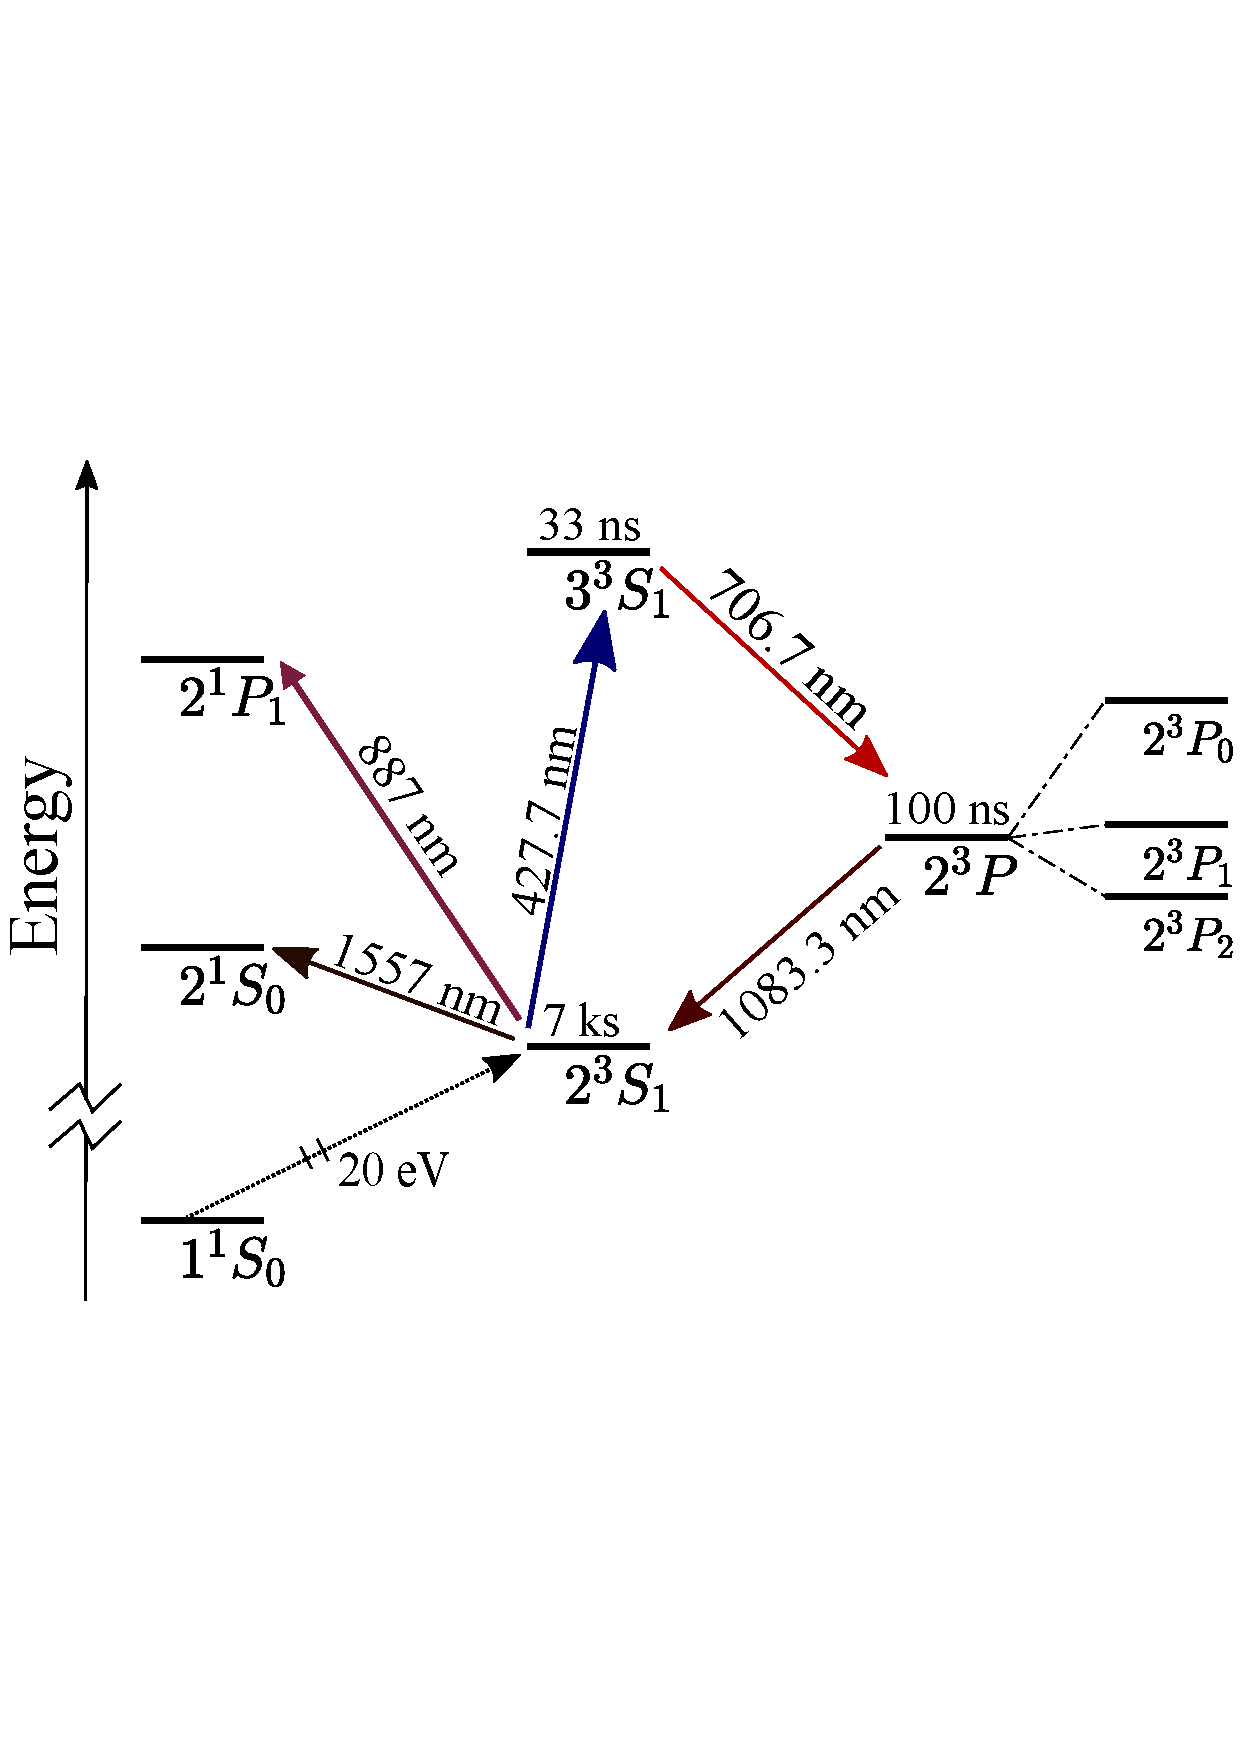
\includegraphics[width=\linewidth]{level_scheme_v5}
    \caption{Partial atomic level scheme for helium. Level splittings are not to scale. The transition of interest, \(\MetastableState \rightarrow \UpperState\), is at \(427.7\)~nm (blue arrow), along with the dominant decay path from the \(\UpperState\) state (\(706.7\)~nm, red arrow). Relevant excited state lifetimes and transition wavelengths are also indicated.
    }
    \label{fig:level_diagram}
\end{figure}

Furthermore, a second extremely weak helium transition of interest is the singlet to triplet ground state transition of metastable helium (He\(^*\)) \(\MetastableState \rightarrow \WimState\)  (see Fig. \ref{fig:level_diagram}), which is doubly forbidden, as it links a triplet to a singlet state, and \(\Delta l = 0\). This transition has a predicted Einstein \(A\) coefficient ranging from $A=6.1\times10^{\text{-}8}$~$\text{s}^{\text{-}1}$ \cite{ISI:000071951300016} to $A=1.5\times10^{\text{-}7}$~ $\text{s}^{\text{-}1}$ \cite{PhysRevA.15.154}, but the transition rate is yet to be measured. 
An experimental measurement of the transition frequency was carried out by van Rooij \textit{et al.} to a precision of \(2\)~kHz for both $^3$He and $^4$He \cite{vanRooij196}. Subsequent measurements by Rengelink \textit{et al.} improved the precision to \(0.2\)~kHz by using a magic wavelength trap \cite{Rengelink2018}, providing a new test of QED and nuclear structure calculations, including a determination of the nuclear charge radius. Of further note are the frequency measurements of seven of the transitions between the \(2^{3\!}S\) and \(2^{3\!}P\) hyperfine manifolds in \(^3\)He by Cancio Pastor \textit{et al.} to the order of \(1\)~kHz \cite{PhysRevLett.108.143001}. This provided a value of the difference of the squared nuclear charge radii of \(^3\)He and $^4$He, which differed by \(4\sigma\) from that derived by van Rooij \textit{et al.}, exemplifying the need to perform different types of experiments to properly constrain QED theory.

%Measurement of the energy separation of this transition was first proposed in \cite{Leeuwen_2006} as a good test of QED, due to the transition being between the singlet and triplet manifolds.
%
%, and because the precision is on the level of nuclear size effects, it can potentially offer new insights into the proton radius puzzle \cite{Pohl2010}.
%


%%%%%%%%%%%%%%%%%%%%%%%%%%%%%%%%%%%%%%%%%%%%%%%%%%%%%%%%%%%%%%%%%%%%%%%%%%%%%%%%%%%%%%%%%%%%%%%

%%Forbidden transitions with isolated upper states are also of particular interest for applications in atomic clocks, as they can possess extremely narrow linewidths, which is a fundamental limit to clock performance. The weakest of these is the electric-octupole transition in \(^{171}\)Yb+  with a corresponding Einstein \(A\) coefficient of \(A = 4(2) \times 10^{\text{-}9}\)~\(\text{s}^{\text{-}1}\) as determined by theory \cite{PhysRevLett.81.3345,PhysRevA.62.020501} (and experiment \cite{PhysRevLett.78.1876}). %, which is only slightly smaller than the Einstein \(A\) coefficient for the \(\MetastableState \rightarrow \UpperState\) transition of interest.
%%Such forbidden transitions have allowed state-of-the-art atomic clocks to be constructed with a relative precision of \(2.5\times 10^{-19}\) \cite{Marti2018}.
%with a state lifetime of \(\text{10}^{+7}_{-4}\text{years}\)
%The Einstein \(A\) coefficient for this transition is predicted to be $A =3.8 \times 10^{\text{-}9} \text{s}^{\text{-}1}$ 
%%%%%%%%%%%%%%%%%%%%%%%%%%%%%%%%%%%%%%%%%%%%%%%%%%%%%%%%%%%%%%%%%%%%%%%%%%%%%%%%%%%%%%%%%%%%%

%\1 we present the measurement of this extremley weak transition in He 4
%\brycecom{This is where we introduce the subject of our study so it should be fairly clear} 
%\brycecom{motivations: dramatic difference in strength prediction, has escaped detection thusfar, its detection advances the methods of forbidden transition metrologoy}

Another transition in helium that until now has not been detected experimentally is the strongly forbidden \(\MetastableState \rightarrow \UpperState\) transition (see Fig. \ref{fig:level_diagram}), for which \(\Delta l = 0\), and it is hence electric dipole forbidden. It is excited via the magnetic dipole interaction using light with a predicted wavelength of \(\sim\)\(427.7\)~nm \cite{Drake2006}. 
There are unresolved conflicting theoretical predictions for the Einstein \(A\) coefficient of this transition. Derevianko \textit{et al.} predict \(A=1.17\times10^{\text{-}8}\)~\(\text{s}^{\text{-}1}\) \cite{PhysRevA.58.4453}, while a calculation by \L{}ach \textit{et al.} gives \(A=6.48\times10^{\text{-}9}\)~\(\text{s}^{\text{-}1}\) \cite{PhysRevA.64.042510}, which states in reference to the differing values \textit{``This discrepancy does not have experimental impact since this rate is too small \ldots to be measured"} \cite{PhysRevA.64.042510}. An accurate measurement of the Einstein \(A\) coefficient for this transition would provide insight into the validity and limitations of the different approaches within QED theory. These calculations also indicate that this transition rate would be the weakest ever measured in a neutral atom, and only slightly stronger than the weakest measured transition rate in an ion: the electric-octupole transition in \(^{172}\)Yb+, which is the longest lived at \(8.4\)~years, \textit{i.e.} \(A = 3.8\times10^{\text{-}9}\)~\(\text{s}^{\text{-}1}\) (theory \cite{PhysRevLett.81.3345}), or \(10^{+7}_{-4}\)~years, equivalently \(A = 3^{+2}_{-1}\times10^{\text{-}9}\)~\(\text{s}^{\text{-}1}\) (experiment \cite{PhysRevLett.78.1876}).
%\(^{172}\)Yb+ with \(A = 4(2)\times10^{\text{-}9}\)~\(\text{s}^{\text{-}1}\) determined by theory \cite{PhysRevLett.81.3345} and observed experimentally by Roberts \textit{et al.} \cite{PhysRevLett.78.1876}.
%The He \(\MetastableState \rightarrow \UpperState\) transition measured here, is of further interest as it is highly sensitive to QED effects \cite{PhysRevA.64.042510}: its first non-zero contributing term to the Einstein \(A\) coefficient is of order \((Z\alpha)^3\) where \(Z\) is the proton number and \(\alpha\) is the fine structure constant. 

%only occurs at third order in QED theory,
%Thus the transition rate is highly sensitive to QED effects \cite{PhysRevA.64.042510}, and

In this work we present the first detection of the \(\MetastableState \rightarrow \UpperState\) transition in $^4$He. We develop two novel techniques for the measurement of ultra-weak transitions and use them to determine the transition frequency,
Einstein \(A\) coefficient and excited state lifetime. The first method uses a Bose-Einstein condensate (BEC) and directly detects atoms which absorb a photon and escape a shallow trap. While this method is highly sensitive and is ideal for the determination of the transition frequency and linewidth, the uncertainty in the collection efficiency necessitates an independent approach for determining the Einstein \(A\) coefficient. To this end we developed a second method, which measures the heating rate of a trapped thermal cloud due to the absorption and subsequent re-emission of photons from a probe beam. From this the Einstein \(A\) coefficient can be extracted. While the use of heating due to photon recoil to detect an excitation has been used for great precision and sensitivity in ion spectroscopy \cite{PhysRevLett.78.1876,Wan2014,PhysRevLett.115.053003,Guggemos_2019} this is the first time such a technique has been utilised in a neutral atom system.
%In general Einstein \(A\) coefficients are  particularly difficult to measure experimentally, especially for weak transitions, and often have large measurement uncertainty. 
%Thus it was important to develop new experimental techniques through which these coefficients can be measured with high accuracy. 
Similar technique could possibly be used to search for other weak transitions which have applications in astronomy and state-of-the-art technologies, such as atomic clocks \cite{detection_note}.

%a RF momentum lens for sensitive detection of the transition frequency and liftime; and a pulsed atom laser heating measurement for measurement of the transition strength. These methods provide a new tool in the search for ultra weak transitions, and cutting edge metrological studies.

%\brycerev{We employ two seperate methods for methods for measuring this transtion.   }

%We develop two novel methods for measuring weak transitions with ultracold \(\MetastableState\) helium atoms

%The resonance measured in the present work is weaker than any other measured atomic transition for neutral atoms, to the best of our knowledge.
%%%%%%%%%%%%%%%%%%%%%%%%%%%%%%%%%%%%%%%%%%%%%%%%%%%%%%%%%%%%%%%%%%%%%%%%%%%%%%%%%%%%%
%We aim to make steps towards resolving this conflict and provide further constraints to QED theory.

%Dumping ground for some other ideas for the intro
%\1 \textbf{Predictions of oscillator strength and how this was thought to be impossible:}

%The oscillator strength of this transition is an excellent testing ground for quantum electrodynamics (QED) theory [\TODO:why?]. . This discrepancy has never been resolved and so we wish to provide an experimental resolution in this work.

%\1 \textbf{other notable forbidden transition in He*:}

%There are a number of recently measured forbidden transitions akin to the one we present here.

%\2 paper that talks about a number of transitions \href{https://www.researchgate.net/publication/287003238_Absorption_at_forbidden_transitions_of_the_helium_atom }{Absorption at forbidden transitions of the helium atom} 


    

%\1 \textbf{forbidden transitions have also been observed by using quadratic fields that have less stringent selection rules \cite{Moore2015}}    

%\1 \textbf{could open a new world of spectoscopy of weak transitions and apply to technologies such as clocks and some other examples:}
%This technique could be applied to the measurement of transitions in thorium and uranium [\TODO:which ones?]. These specific transitions are of great interest as they are excellent candidates for clock transitions. [\TODO:why?]
%Forbidden transitions as play an important role in metrology and astronomy as frequency standards \cite{} [\TODO:expand].



%marked with its approximate wavelength of
%\section{Direct Detection of the Transition Frequency}
%\begin{outline}[enumerate]
%\1 \textbf{He* production (laser cooling etc) + Our trap and its paremeters:}

%\brycecom{both experiments dont start with a BEC}
%\brycecom{reference previous experiments for the technical details, in particular ML, BCR}
To measure the transition frequency and linewidth we start with a BEC of \(\sim\)\(10^6\) He\(^*\) atoms trapped in the long-lived \(\MetastableState\) excited state \cite{PhysRevLett.103.053002}, prepared via a combination of laser and evaporative cooling in a magnetic bi-planar quadrupole Ioffe trap \cite{Dall2007}. The atoms are prepared in the \(m_J=+1\) magnetic substate, as this is the only magnetically trapped state \cite{Dall2007}. The atoms are detected after falling onto an 80 mm diameter micro-channel plate and delay line detector (DLD) \cite{Manning:10} (see remark \cite{detection_note} for extensions to other atoms), located approximately 850 mm below the trap centre (Fig.~\ref{fig:exp_setup}). 
%to determine the cloud temperature, which is far less sensitive.
%, which has trapping frequencies \(\omega_{(x,y,z)}/2\pi=\big(53.5(6),426.56(5),430.30(6)\big)\)~Hz
%majorana losses are suppressed by a strong bias, and polarization suppresses Penning losses (it's also the only state of He* that can be magnetically trapped, because the no-source theorem prevents a local maximum that would be needed to trap the -1 state).
% as this is the only magnetically trapped state.
%to avoid Majorana spin flip losses

To address the \(\MetastableState \rightarrow \UpperState\) transition we illuminate the atoms with a probe beam from a laser and doubling cavity that is tuneable around 427.7nm \cite{SOMs}.  The frequency of the laser was stabilised using a feedback loop to a wavemeter with \(2\) MHz absolute accuracy, which was periodically calibrated to a known cesium crossover transition (see \cite{SOMs} for further detail). After passing through an optical fibre, the probe beam is focused and aligned along the weak axis of the trap, see Fig.~\ref{fig:exp_setup} for diagram of experimental setup. We then perform differential measurements between the laser applied and a reference shot with the laser blocked.
%from \(6^2S_{\nicefrac{1}{2}}, F=4\) to between \(6^2P_{\nicefrac{3}{2}}, F=4\) and \(6^2P_{\nicefrac{3}{2}}, F=5\)
%, constrained to be \(351,721,835.0(1)\)~MHz \cite{pmid9900545}
%. This cesium transition was chosen as it is close to the predicted frequency of the transition before doubling \(350,469,635(4)\)~MHz \cite{Drake2006}.

\begin{figure}[t]
\includegraphics[width=\linewidth]{exp_diag_v4.png}%{3d_schematic.png}% Here is how to import EPS art
\caption{\label{fig:exp_setup}Diagram of the experimental setup. A BEC is produced and then held in a magnetic trap. The laser light is focused onto the atoms in the trap and when an atom absorbs one of the photons it will most likely leave the trap, with some high probability of it landing on the detector.}
\end{figure}



%and the ground-state values which are exact due to the current definition of the second \cite{}.

%\1 \textbf{explanation of RF outcoupling and the dld (single atom detection):}


%The large internal energy of the 23S1 state of He* (∼20 eV) allows the DLD to reconstruct individual atoms at a spatial resolution of ∼120 µm, a temporal resolution of ∼3 µs (see Appendix B) and a quantum efficiency of ∼10%.

%\1 \textbf{The beam and how we regulate it:} 



%\1 \textbf{Trap freq method (cite trap freq metrology paper), How we use this to align the beam, and measure the density distribution of the BEC:}

%\subsection{method description}
%\brycecom{explain difficulties with osc stength method}
The transition is detected by directly measuring small numbers, on the order of \(10^2\), of atoms that absorb the probe laser light during a \(25\)~s exposure time. 
When the wavelength of a \(\sigma^-\) polarised probe laser beam is resonant with the \(\MetastableState \rightarrow \UpperState\) transition, the \(427.7\)~nm photon excites the atom from the \(\MetastableState , m_J=+1\) state to the \(\UpperState , m_J=0\) state and the atom receives a momentum recoil. 
%\brycecom{calculate the loss rate to other paths}
%\brycerev{The dominant decay path (xx loss to other paths) is via two subsequent photon emissions, first emitting a 706~nm photon to one of the \(\MidState\) states  (\(\tau \sim\)~170~ns) and in turn emitting a 1083~nm photon to the \(\MetastableState\) state ( \(\tau \sim\)~100~ns). Based on the Clebsch-Gordan coefficients an atom initaly in the mj=1 state that absorbs a (pi/sigma) photon will have a probability of (1/x,1/x,1/y) in the mj (-1,0,1) state respectively. }
%\brycecom{i would prefer the exact fractions here}
The vast majority of these excited atoms then decay within $\sim$30~ns, emitting a photon at \(706.7\)~nm to one of the \(\MidState\) states, then within $\sim$100~ns decay via the \(1083\)~nm transitions to the \(\MetastableState\) state (see Fig.~\ref{fig:level_diagram}). This is because all other transitions from \(\UpperState\) and the \(\MidState\) states are forbidden: hence less than 1 in \(10^4\) atoms will decay to non-\(\MetastableState\) states \cite{PhysRevLett.100.023001,Hodgman2009a}.
%to \(2^{1\!}S_0\), \(\MetastableState\), and \(1^{1\!}S_0\), as well as transitions from the
% to \(\GroundState\) and \(2^{1\!}S_0\)

%initially in the magnetically trapped \(\MetastableState, \, m_J=+1\) state that absorb a \(427.7\)~nm probe beam photon, polarised to excite a $\sigma^-$ transition,
Atoms will hence on average end up distributed among the magnetic sublevels \(m_J=(-1,0, 1)\) of the \(\MetastableState\) state with a fractional population of (24\%,52\%,24\%) based on the relevant transition Clebsch-Gordan coefficients. 
The 76\% of atoms that decay to the untrapped \(\MetastableState, \, m_J=0\, \text{or} \, -1\) states leave the trap immediately and fall under the influence of gravity onto the DLD, with the chance that they will collide with other atoms while leaving the BEC \cite{SOMs}. %another \(427.7\)~nm photon or
\begin{figure}[b]
\centering
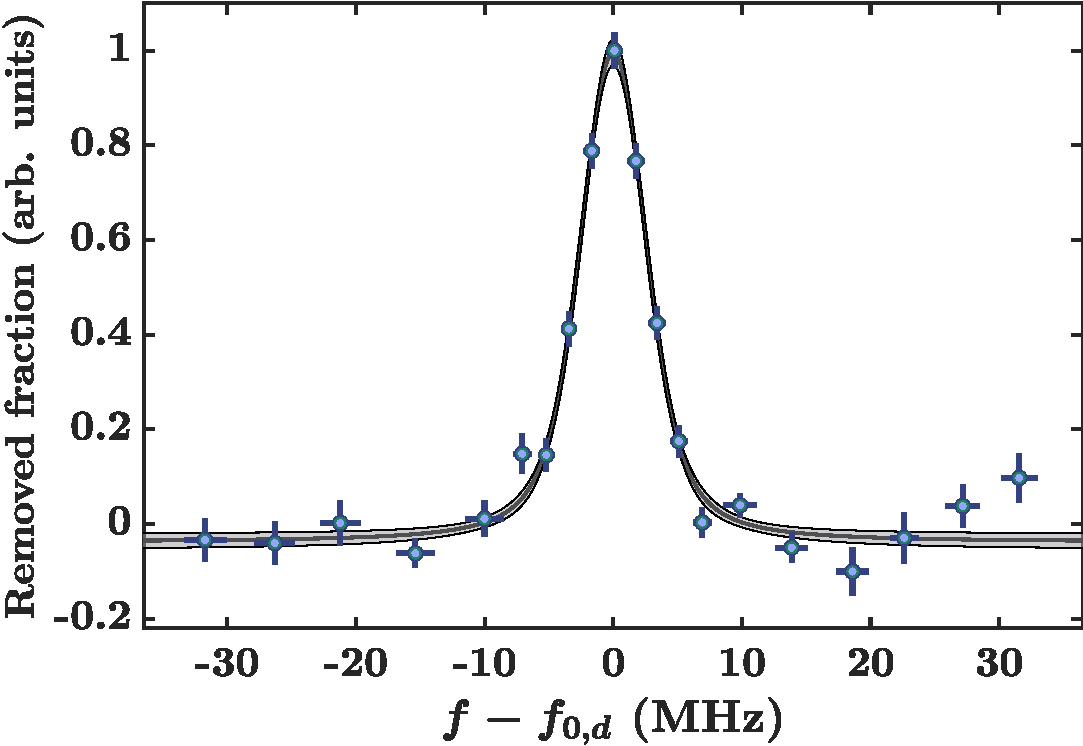
\includegraphics[width=\linewidth]{direct_scan_voigt_full_v4}
\caption{(Color online) The normalised excited fraction as a function of applied laser frequency (relative to the fitted centered frequency \(f_{0,d} = 700,939,271.64(8)\)~MHz where quoted error is purely statistical). Vertical and horizontal bars indicate the uncertainty in their respective axis \cite{standard_error_note}. Data has been binned for viewing, where the width of the bin used to calculate each point is varied to compensate for the varying density of sample points. The black line is a Voigt fit to the data, with the grey shaded region indicating the confidence interval.  The parameters of the fit are \(\sigma=1.9(4)\)~MHz (standard deviation of the Gaussian component) and \(\gamma=3.2(10)\)~MHz (scale parameter of the Lorentzian component), corresponding to an excited state lifetime of \(50(20)\)~ns. The peak signal represents an excited fraction of 0.34\% for a total energy of applied photons of \(0.65\)~J.
}
\label{fig:427nm_signal}
\end{figure}

% The parameters of the fit are \(\sigma=0.67(14)\)~MHz (standard deviation of the Gaussian component) and \(\gamma=5.4(5)\)~MHz (scale parameter of the Lorentzian component), corresponding to an excited state lifetime of ...
%The full width at half maximum of the fit is {\color{red} \(5.7(3)\)~MHz, corresponding to an excited state lifetime of \(33(6)\)~ns.

%\brycerev{The two subsequent photon decays produce a momentum distribution which is a filled shell with a center translated by and an outer radius equal to a 427~nm photon recoil.}
%\brycecom{describe the momentum spcae distribution of the atoms after the two photon decays}
%($\sim$ 24\%) will return to the trapped
%over unscattered atoms
The remaining \(24\%\) of excited atoms that have decayed to the \(\MetastableState, m_J=+1\) state will be re-trapped.
%with increased momentum from the photon recoil. By applying RF radiation tuned to the \(\MetastableState, m_J=1 \rightarrow 0\) transition for a given magnetic field strength we can selectively outcouple these higher energy atoms, as the maximum magnetic field experienced by an atom is proportional to its maximum kinetic energy \cite{SOMs}.
%As the maximum magnetic field experienced by an atom oscillating in the magnetic trap is proportional to its maximum kinetic energy, by applying RF radiation tuned to the \(\MetastableState, m_J=1 \rightarrow 0\) transition for a given magnetic field strength we can selectively outcouple atoms with maximum kinetic energy above a threshold. Furthermore, as an atom does work on the trap the momentum space distribution of these outcoupled atoms is reduced in size, hence improving collection efficiency. Thus while only $\sim$ 24\% of atoms decay to the \(\MetastableState, m_J=+1\) state via this process they can significantly increase the total signal amplitude \cite{SOMs}. The interplay between these two effects produce an optimum collection efficiency that depends on the particular momentum distribution and detector geometry.
%For our case we found this optimum to be \(2.05\)~MHz above the minimum magnetic field strength in our trap, known as the trap bottom. Note that this RF radiation is far detuned from the momentum width of the BEC plus the trap bottom, and so should remove a negligible number of atoms from the original BEC momentum distribution. 

%All outcoupled atoms (through either optical scattering or optical and RF outcoupling) then fall under gravity and are detected on the DLD.

%All the atoms that have experienced scattering into any \(\MetastableState\) magnetic sub-level will thereby be outcoupled (through either optical scattering or optical/RF outcoupling), and will then fall under gravity onto the DLD.

%Monte-Carlo simulations show that in total atoms have a \(xx\) \% chance of hitting the detector \cite{SOMs}.  , showing that our method is able to detect small numbers of scattered atoms.

%

%\1 \textbf{The laser is locked to a wm using a pid feedback loop, the wm itself is periodically calibrated to a transtion wich is x~nm's away, we create a drift model using these calibrations inorder to correct for the wm drift}



%\1 \textbf{Explanation of why we used two separate methods:}

%In order to detect and characterise the \(\MetastableState \rightarrow 3^3S_1\) transition we employ two separate methods, the direct detection and heating methods. The reason for each method is: the direct detection method is more sensitive, while the heating method allows us to measure the oscillator strength of the transition. Furthermore it provides two independent measurements of the transitions frequency and width.
%\1 \textbf{RF knife and direct detection:}


%\2 k-space description and multiscatterinng, spilling over the RF knife, then some proportion hitting the detector.
%k-space description




%Monte Carlo simulation to determine that proportion (so we can extract an estimate of the oscillator strength)


%\brycecom{To measure the total number while preventing saturation of our detector}
After the probe beam is switched off, the remaining atoms in the magnetic trap are outcoupled with pulses of broadband RF radiation.
%radio frequency (RF) radiation resonant to the Zeeman splitting between the \(m_J=+1\) (trapped) and \(m_J=0\) (untrapped) magnetic sublevels. uniformly
This transfers all atoms from the trap into a coherent beam of atoms, known as an atom laser \cite{Manning:10,Henson2018}, allowing the total number of remaining atoms in the trap to be measured, while avoiding detector saturation. The ratio of excited and lost atoms to remaining atoms can hence be determined, which is less sensitive to total BEC number fluctuations from shot-to-shot.

%\subsection{Results}

%There is a negative offset from zero in the data that has a p-value of \(8.4 \times 10^{-7}\), and could be caused by dipole trapping of atoms.
% The peak signal corresponds to a scattered fraction of 0.34\% for an integrated power of \(6.5 \times 10^{-4} \, kJ\).
%\brycecom{to calibrate the effect/affect of the probe laser, we perform every nth shot with the laser off} 
For each laser wavelength, \(\sim\)\(215\) shots are taken with the probe beam applied and \(\sim\)\(50\) with it blocked as a reference, from which the normalised excitation probability per photon per unit time \cite{SOMs} is extracted. The excited fractions for a range of frequencies around the transition are shown in Fig.~\ref{fig:427nm_signal}.  At resonance, we measure a peak signal corresponding to 0.34\% of the total atoms excited per \(\sim\)\(10^{18}\) applied photons (for details on the beam shape and power in relation to the atom sample see \cite{SOMs}).  Note that the signal in Fig.~\ref{fig:427nm_signal} decays to a negative value far from the transition.  We speculate that this is due to the off-resonant repulsive dipole potential of the probe beam on the atoms, which causes a deflection of atoms such that they miss the detector, compared to the reference case.  While this effect is measurable, it has a negligible effect on the line shape compared to the other sources of error \cite{SOMs}. 

%sensitivity
%the signal to noise ratio scales as \(0.0017/\sqrt{\text{atom J}}\) and so \(A_{min} = 8.3\times10^{\text{-}6}\)~\(\text{s}^{\text{-}1}\sqrt{\text{atom J}}\), and
%a sensitivity metric , which indicates
%of approximately \(10^6\) atoms, and \(0.65\times 215\)~J total time integrated power,

%%%%%%%%%%%%%%%%%%%%%%%
%%%%%%%%%%%%%%%%%%%%%%%
%We can calculate for this method the weakest detectable transitions as characterised by \(A_{min}\), for a given power, atom number, and interrogation time \cite{SOMs}. We find for our specific case \(A_{min}\sim 5\times10^{\text{-}10}\)~\(\text{s}^{\text{-}1}\).
%%%%%%%%%%%%%%%%%%%%%%%
%%%%%%%%%%%%%%%%%%%%%%%

The centre of the corresponding Lorentzian fit gives a measured transition frequency of \(f_{0,d}=700,939,271.64(8)\)~MHz, with subscript \(d\) referring to the direct detection method and with only the statistical uncertainty shown.  After applying relevant systematic corrections (as listed with the full error budget in Tab.~\ref{tab:corrections}), this yields a final value of \(f_{0,d}^{shifted}=700,939,271(5)\)~MHz.  This agrees very well with the most recent published value in the literature of \(700,939,269(8)\)~MHz \cite{Drake2006}, with our uncertainty smaller than that of theory.  The Lorentzian width of the peak, derived from the Voigt fit (see Fig.~\ref{fig:427nm_signal}), also allows the state lifetime of the $3^{3\!}S_1$ state to be determined.  We estimate an excited state lifetime of \(\tau = 50(20)\)~ns, which compares well to the theoretical value of \(35.9(2)\)~ns \cite{SOMs}. We also find that the sensitivty of this method is such that an Einstein \(A\) value of \(\approx 7 \times10^{-11}\)~\(\text{s}^{\text{-}1}\) could be observed with a SNR of unity given one day of interrogation \cite{SOMs}.
%, once external systematic effects such as laser power broadening are removed 
%, maybe think some more whey this could be the case, maybe reduced density of the could reduces penning ions a back of the envelope would be helpful }


%this stuff should be accounted for in doppler right?
%
% \begin{table*}[b]
%     \centering
%     \begin{tabular}{|l|r|r|r|r|}
%         \hline
%         &\multicolumn{2}{c|}{\(f_{0,d}\)}&\multicolumn{2}{c|}{\(f_{0,h}\)}\\
%         \hline
%         Value & Systematic & Unc (MHz)& Systematic & Unc (MHz)\\
%         & Freq Shift (MHz) & & Freq Shift (MHz) &\\
%         \hhline {|=====|}
%          Zeeman shift & -1.7154 & 0.003 & -1.7154 & 0.003 \\
%          AC Stark shift &&&&\\%\cite{Delone_1999}
%           \, \, - Probe & 8.57& 1.5 & & \\
%           \, \, - RF knife & 0.94 & 1.8 & & \\
%          DC Stark shift  &negligible & 00 &negligible & 00\\% \cite{Delone_1999}
%          Mean field shift & negligible & 00& negligible & 00\\%\cite{PhysRevLett.81.3807}
%          Recoil shift & 0.273 & 00 & 0.273 & 00  \\
%          Cs Cell offset & & &&\\
%          \, \, - AC Stark shift & -1.88 & 0.43 & -1.88 & 0.43\\
%          \, \, - Pressure shift & negligible & 00 & negligible & 00 \\ %\cite{mcguyer_phdthesis}
%          Wavemeter & 0 & 4.0 & 0 & 4.0\\
%          Statistical & 0 & 0.08 & 0 & 0.6\\
%          \hline
%          Total & 6.2 & 4.7 & &\\
%          \hline
%     \end{tabular}
%     \caption{Systematic shifts, corrections, and uncertainties to measured frequency values from the direct detection method \(f_{0,d}\) and the heating method \(f_{0,h}\). Note that uncertainties are added in quadrature.}
%     \label{tab:corrections}
% \end{table*}

\begin{table}[b]
    \centering
    \begin{tabular}{@{\extracolsep{\fill}} l @{\extracolsep{\fill}}>{\centering}p{0.09\textwidth} @{\extracolsep{\fill}}>{\centering}p{0.09\textwidth} @{\extracolsep{\fill}}>{\centering}p{0.07\textwidth} @{\extracolsep{\fill}}>{\centering\arraybackslash}p{0.07\textwidth}}
    \toprule
    \toprule
        Value & \multicolumn{2}{c}{Systematic} & \multicolumn{2}{c}{Unc (MHz)}\\
        &\multicolumn{2}{c}{Freq Shift (MHz)}&\multicolumn{2}{c}{}\\
        \hline
         &\(f_{0,d}\)&\(f_{0,h}\)&\(f_{0,d}\)&\(f_{0,h}\)\\
        \hline
         Zeeman shift &\multicolumn{2}{c}{ \(-1.715\) } & \multicolumn{2}{c}{0.003} \\
         AC Stark shift & 6.9 &5.9  & 1.5 & 1.6\\
          %\, \, - Probe & 6.9 & 5.9  & 1.5 & 1.6 \\
          %\, \, - RF knife & 0.94 &  0 & 1.8 & 0\\
         DC Stark shift & \multicolumn{2}{c}{\(<10^{-6}\)} & \multicolumn{2}{c}{-}\\
         Mean field shift & \multicolumn{2}{c}{\(<0.01\)} & \multicolumn{2}{c}{-}\\
         Recoil shift & \multicolumn{2}{c}{0.273}  & \multicolumn{2}{c}{\(<\)0.001}  \\
         Cesium Cell offset & \multicolumn{2}{c}{} & \multicolumn{2}{c}{}\\
         \, \, - AC Stark shift & \multicolumn{2}{c}{\(-1.9\)} & \multicolumn{2}{c}{0.4} \\
         \, \, - Pressure shift & \multicolumn{2}{c}{\(<0.006\)} & \multicolumn{2}{c}{-} \\
         Wavemeter & \multicolumn{2}{c}{\(-3.0\)} & \multicolumn{2}{c}{4.1}\\
         Statistical & \multicolumn{2}{c}{-}  & 0.08 & 0.6\\
         \hline
         Total & 0.6 & -0.4 & 4.4 & 4.5\\
    \bottomrule
    \bottomrule
    \end{tabular}
    \caption{Systematic shifts, corrections, and uncertainties to measured frequency values from the direct detection method \(f_{0,d}\) and the heating method \(f_{0,h}\). Note that uncertainties are added in quadrature.}
    \label{tab:corrections}
\end{table}

%\section{Heating Detection for Measurement of Transition Strength}
%\1 \textbf{Heating method and such:}
%\2 How we determine the temperature (out coupling RF pulses and thermal Boltzmann fit, Gaussian)

To measure the transition strength, we employ a different experimental technique that determines the heating of the cloud induced by the photon recoil of absorbed and emitted photons from the probe beam. The thermal cloud has an initial temperature of order \(1\)~\(\mu\)K.  We use a minimally-destructive spectrally broad RF pulse to remove \(\sim\)2\% of the atoms from the trap. The pulses are approximately 20~\(\mu\)s in length, and hence have a Fourier width of \(\sim 300\)~kHz \cite{Manning:10}, which ensures uniform outcoupling throughout the trap. The time-of-flight profile recorded on the DLD in the far field will represent the momentum profile of the trapped atoms \cite{Yavin2002}. As the temperature of the atoms is significantly above the condensation temperature, \(T_c \sim 150\)~nK, the temperature was found by fitting each profile with a Boltzmann distribution \cite{SOMs}.
%this profile is well approximated by a Boltzmann distribution. Hence
%, as displayed in Fig.~\ref{fig:427nm_signal_heating}, 
%a Gaussian fit to a single outcoupled pulse of atoms provides a temperature measurement of the cloud at that point in time.   
%
%\2 Use heating rate (change of temp over time) to account for fluctuation in initial temp
\begin{figure}[t]
    \centering
    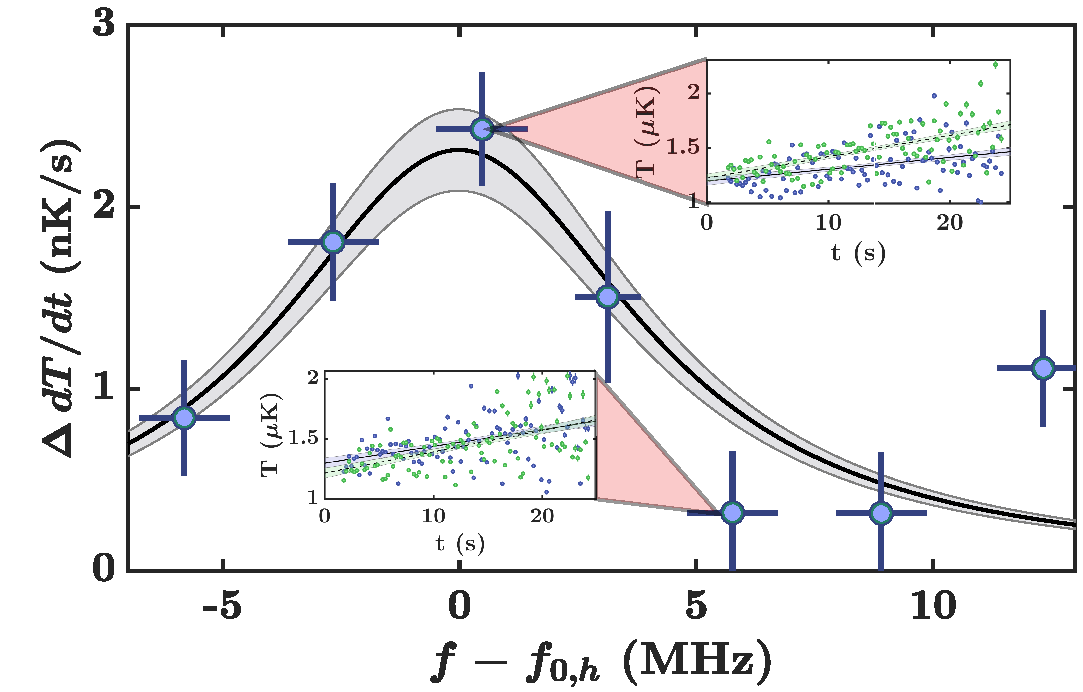
\includegraphics[width=\linewidth]{heating_scan_voigt} % second figure itself
    \caption{(Color online) Increase in heating rate as a function of applied laser frequency, relative to fitted frequency center \(f_{0,h} = 700,939,270.9(6)\)~MHz, with quoted error purely statistical. Data has been binned in frequency for clarity, with vertical and horizontal bars indicating uncertainty in the respective axis \cite{standard_error_note}. The solid black line represents a Voigt fit with \(\sigma=1.6(9)\)~MHz, and \(\gamma=4(3)\)~MHz. The insets show a comparison of heating rates at the respective frequencies, with the dashed (green) line indicating a run with the laser light applied and the solid (blue) line indicating a reference run.
    }
    \label{fig:427nm_signal_heating}
\end{figure}
By repeatedly outcoupling small numbers of atoms (the full sequence uses 95 pulses each spaced 240~ms apart), the temperature of the trapped thermal cloud can be estimated as a function of time, and thus a heating rate determined. Comparison of the measured heating rate when the probe beam is present to when it is blocked allows an estimate of the heating rate due to the probe beam.  The difference in the heating rates between probe and reference is shown in Fig.~\ref{fig:427nm_signal_heating} as a function of laser frequency, which gives a fitted peak frequency for this method of \(f_{0,h}^{shifted}=700,939,270.9(6)\)~MHz, (with subscript \(h\) referring to the heating method, and with the statistical uncertainty shown). After applying appropriate systematic frequency shifts (see Tab.~\ref{tab:corrections} \cite{SOMs}), the final value for the transition frequency is \(f_{0,h} = 700,939,271(5)\)~MHz, and the excited state lifetime is \(40(30)\)~ns. Both agree within uncertainty with the values measured by the direct detection method.

We calculate the Einstein \(A\) coefficient from the measured heating rate and the heat capacity of a harmonically trapped Bose gas \cite{SOMs}. The resultant value is \(A =7(4)\times 10^{\text{-}9}\)~\(\text{s}^{\text{-}1}\), compared to the most recent theoretical value of \(A=6.48\times 10^{\text{-}9}\)~\(\text{s}^{\text{-}1}\) \cite{PhysRevA.64.042510}.
%\2 From heat added we can calculate number of photons scattered and from that oscillator strength and integrated width to remove broadening in osc strength calculation.
%\1 We periodically take shots with no laser to calibrate our signal (the calibration shots) from this we create a drift/cal model
%\end{outline}
%A_min_disc
%%%%%%%%%%%%%%%%%%%%%%%%%%%%%%%%%%%%%%%%%%%%%%%%%%%%%%%%%%%%%%%%%%%%%%%%%%%%%%%%%%%%%%%%%%%%%%
%For reference we find the weakest transitions the heating method could ideally detect, based upon the statistical uncertainty in the data and for our experimental conditions, to be \(A_{min} \sim 1.8\times10^{\text{-}9}\)~\(\text{s}^{\text{-}1}\) \cite{SOMs}. %The absolute value of this fundamental limiting sensitivity is far below that of other techniques, which historically have had similar relative uncertainties of \(25\%\) to \(50\%\) but absolute uncertainties of \(\sim10^{3}\)~\(\text{s}^{\text{-}1}\) \cite{Whaling85,Pickering11}. 
%%%%%%%%%%%%%%%%%%%%%%%%%%%%%%%%%%%%%%%%%%%%%%%%%%%%%%%%%%%%%%%%%%%%%%%%%%%%%%%%%%%%%%%%%%%%%%
%Using the same method as for the direct detection, w

%\section{Discussion and Conclusion}
\renewcommand\arraystretch{1.3}
\begin{table}[b]
    \centering
    \begin{tabular}{@{\extracolsep{\fill}} l @{\extracolsep{\fill}} c @{\extracolsep{\fill}} c @{\extracolsep{\fill}} c}
    \toprule
    \toprule
         \multicolumn{1}{l}{Method} & \multicolumn{1}{c}{Center}  & \multicolumn{1}{c}{\(\UpperState\) State}  & \multicolumn{1}{c}{Einstein \(A\)}  \\
          & \multicolumn{1}{c}{Freq (MHz)} & \multicolumn{1}{c}{Lifetime (ns)} & \multicolumn{1}{c}{Coeff (\(10^{\text{-}9}\)s\(^{\text{-}1}\))}\\
         \hline 
         Direct & \(700,939,271(5)\) & \(50(20)\) & - \\
         Heating & \(700,939,271(5)\) & \(40(30)\) & \(7(4)\) \\
         Theory & \(700,939,269(8)\)\cite{Drake2006} & \(35.9(2)\)\cite{SOMs} &\(6.48\)\cite{PhysRevA.64.042510}, \(11.7\)\cite{PhysRevA.58.4453}\\
          %&&&\\
    \bottomrule
    \bottomrule
    \end{tabular}
    \caption{Summary table of experimentally measured values, including all systematic corrections, for the \(\MetastableState \rightarrow \UpperState\) transition in Helium, with the most recent theoretical calculations for comparison.}
    \label{tab:summary}
\end{table}

%talk about our results
Our results for the transition frequency using both methods compare well with the most recent theoretical value in the literature (see Tab.~\ref{tab:summary}), and our experimental uncertainty is comparable to that of the current QED theory calculation.  A further consequence of our measurement of the \(\MetastableState \rightarrow \UpperState\) transition wavelength is that it constrains the \(2^{3\!}P_1 \rightarrow \UpperState\) transition frequency to be \(424,202,774(5)\)~MHz, using the extremely accurately measured \(\MetastableState \rightarrow 2^{3\!}P_1\) transition frequency \cite{PhysRevLett.119.263002}. Further, the experimental Einstein \(A\) coefficient also agrees within error with both of the most recent theoretical published values \cite{PhysRevA.58.4453,PhysRevA.64.042510}, although it is not sufficiently sensitive to resolve the difference between them. Nonetheless, the measurement of transition strengths is important as an alternative test for QED, as there are few techniques which can be compared to energy level measurements, and thus further investigation is warranted.
%A_min_disc
%However, our limiting sensitivity is far below the discrepancy between the two (\(1.8\times10^{\text{-}9}\)~\(\text{s}^{\text{-}1}\) compared to \(5.2\times10^{\text{-}9}\)~\(\text{s}^{\text{-}1}\)), thus further measurements could resolve the two providing insight into the validity of the conflicting approaches used to calculate the theoretical values. 
%conclusively %However, with more research we would able to reach our limiting sensitivity of Amin, and would hence be able to resolve the descrepencay  

In conclusion, we have demonstrated a novel sensitive method for measuring and characterising spectroscopic transitions in helium that could in principle be extended to other metastable atoms, particularly those that are used in ultracold gas experiments \cite{RevModPhys.84.175}. This has allowed us to detect the weakest transition ever observed in a neutral atom.  The techniques are based upon momentum detection of atoms, separating them from most other techniques in the literature which are usually based upon measuring change in irradiance.  While our method agrees within experimental uncertainty with theory, by increasing the accuracy of the laser wavelength measurement  (e.g. via incorporating a frequency comb), we could reach a level of accuracy of \(<1\)~MHz, which would provide a challenge to improve state-of-the-art theoretical predictions.  Furthermore, by conducting similar measurements on $^3$He, isotope shifts could also be compared as a further test of QED predictions.
%Applications to new technologies (what are they?)
%atom_clocks
%%%%%%%%%%%%%%%%%%%%%%%%%%%%%%%%%%%%%%%%%%%%%%%%%%%%%%%%%%%%%%%%%%%%%%%%%%%%%%%%%%%%%%%%%%%
%might remove or swap with the paragraph below
%We have also found that the limiting sensitivity of our techniques is far below that of other such techniques used to measure Einstein \(A\) coefficients \cite{Whaling85}. The high sensitivity of our technique for extremely weak transitions in principle could be extended to measure weak transitions in other atoms, which are important in precision metrology and astronomy \cite{Pickering11}. A key application of weak transitions is to atomic clocks, and our techniques could be extended to search for new clock transitions, such as the nuclear clock transition in %$^{229}$
%thorium \cite{Campbell2012,vonderWense2016,vonderWense2018,Seiferle2019}. 

%{\color{red} As stated above the ability of our techniques to detect extremely weak transitions in principle could be extended to measure weak transitions in other metastable atoms, particularly those used in ultracold experiments \cite{RevModPhys.84.175}.}
%%%%%%%%%%%%%%%%%%%%%%%%%%%%%%%%%%%%%%%%%%%%%%%%%%%%%%%%%%%%%%%%%%%%%%%%%%%%%%%%%%%%%%%%%%%
%, and could extend further to detect transitions as weak as \(A_{min} \sim 1.8\times10^{\text{-}9}\)~\(\text{s}^{\text{-}1}\),
%\end{outline}
%\\ \\


\begin{acknowledgments}
The authors would like to thank G. W. F. Drake, G. \L{}ach and K. Pachucki for helpful discussions, and C. J. Vale and S. Hoinka for the loan of the laser.
This work was supported through Australian Research
Council (ARC) Discovery Project Grants DP160102337 and DP180101093, %ken tune out DP 
as well as Linkage Project LE180100142.
K.F.T. and D.K.S. are supported by Australian Government Research Training Program (RTP) Scholarships.
S. S. H. is supported by ARC Discovery Early Career Researcher Award No. DE150100315.
\end{acknowledgments}


\bibliography{forbidden427}% Produces the bibliography via BibTeX.
\end{document}
%
% ****** End of file apssamp.tex ******
